% \newpage
% 
% \onecolumn
% 
% \appendix
% 
% \section{Oszilloskop-Bilder}
% \label{sec:plots}
% \begin{figure}[htbp]
% \begin{center}
%   \subfloat[Photomultiplier 1]{
%     \label{fig:photomultiplier_1}
%     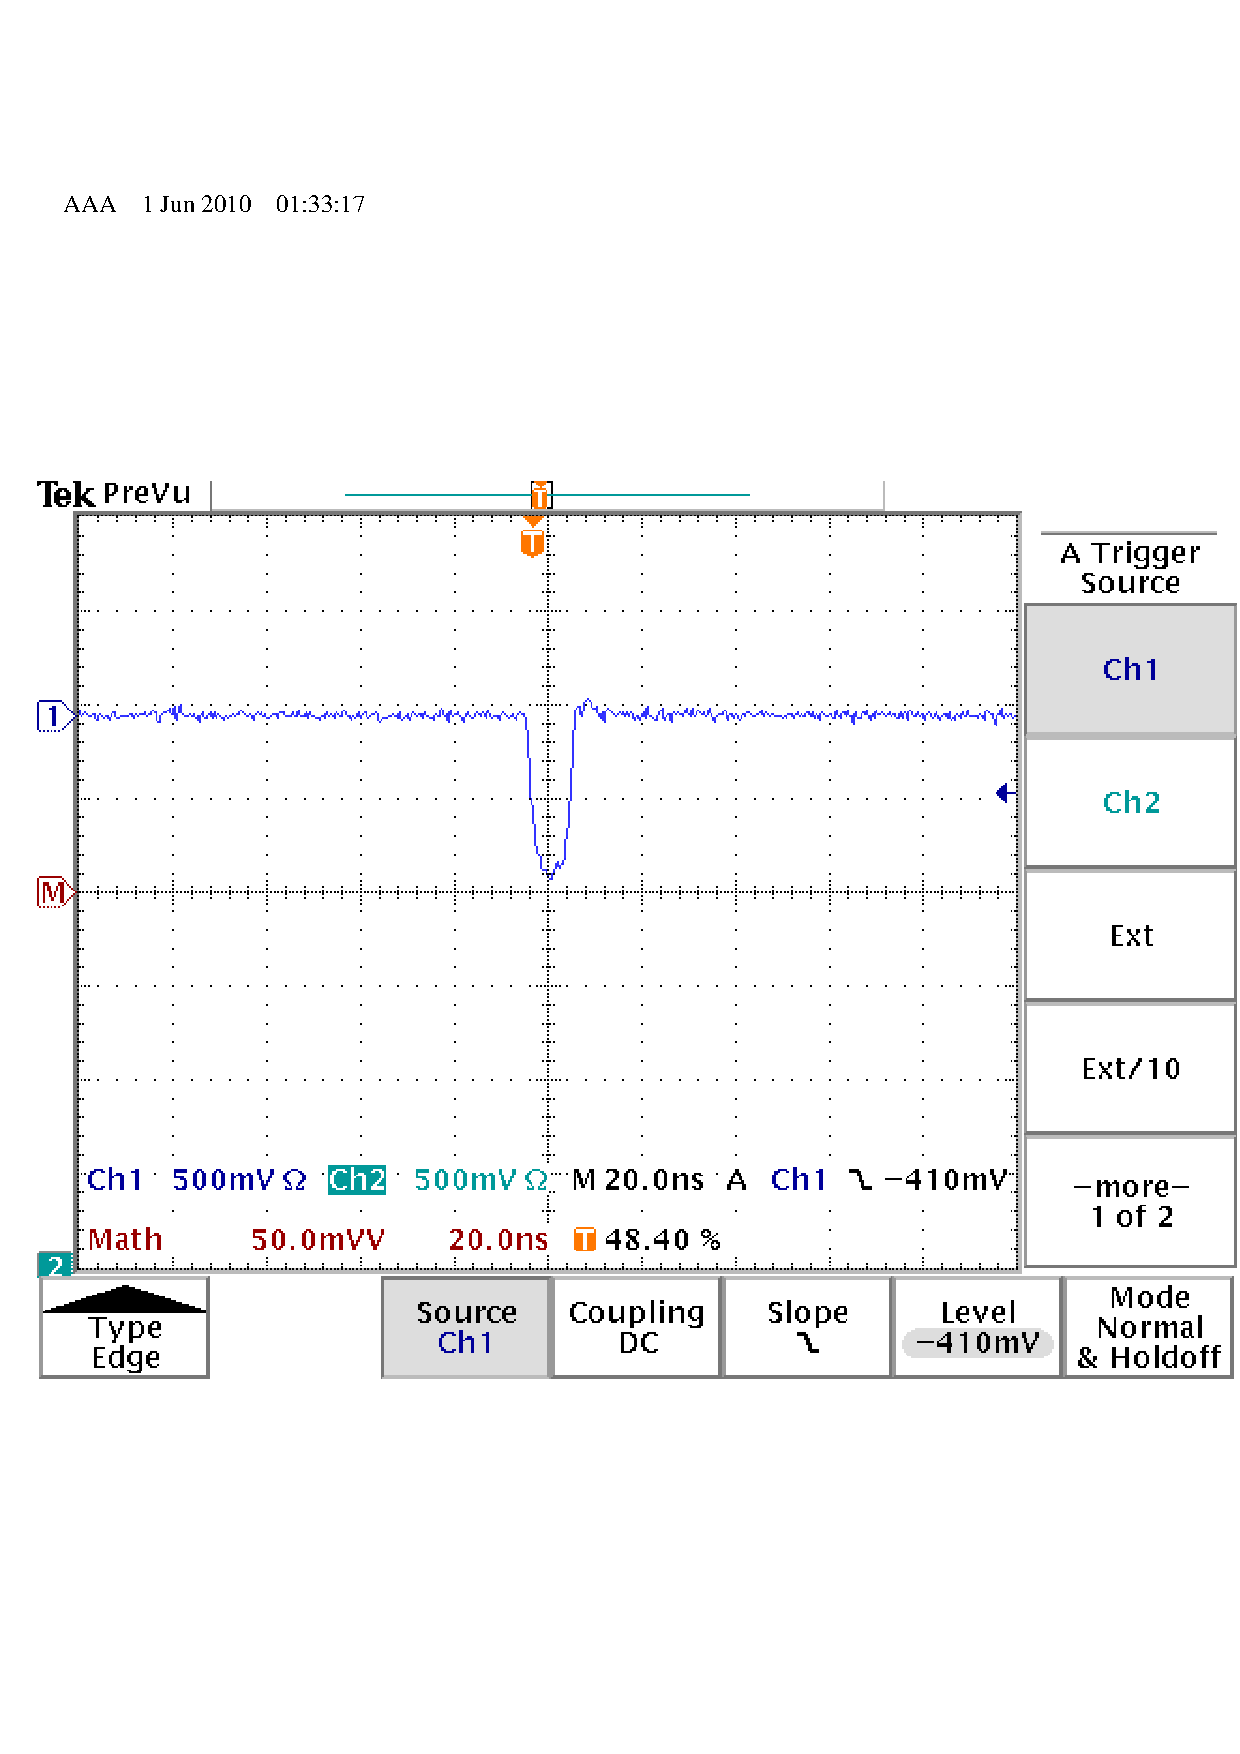
\includegraphics[width=0.45\textwidth,keepaspectratio,viewport=0 52 472 436,clip]{../tmp/TEK00013.pdf}}
%   \subfloat[Photomultiplier 2]{
%     \label{fig:photomultiplier_2}
%     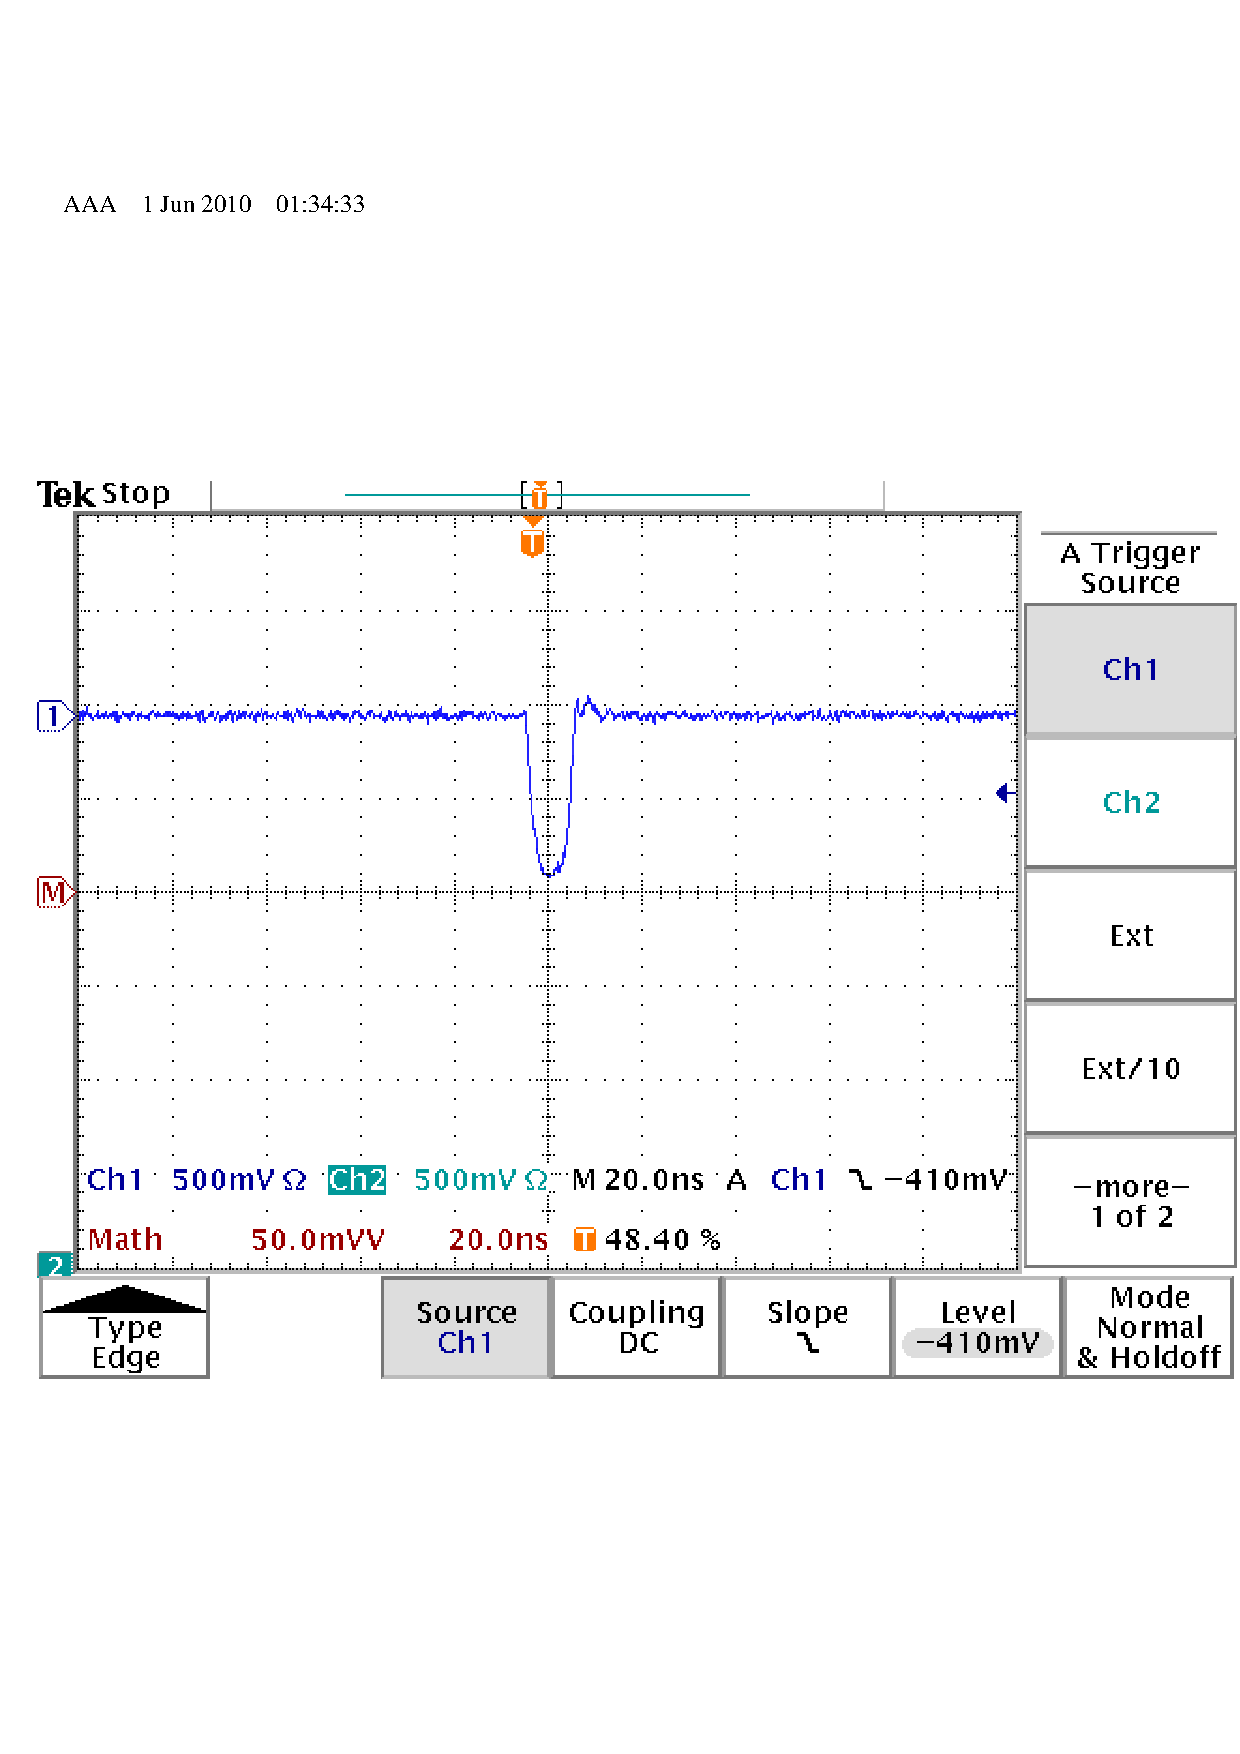
\includegraphics[width=0.45\textwidth,keepaspectratio,viewport=0 52 472 436,clip]{../tmp/TEK00014.pdf}
%   }
%   \newline
%   \subfloat[Photomultiplier 3]{
%     \label{fig:photomultiplier_3}
%     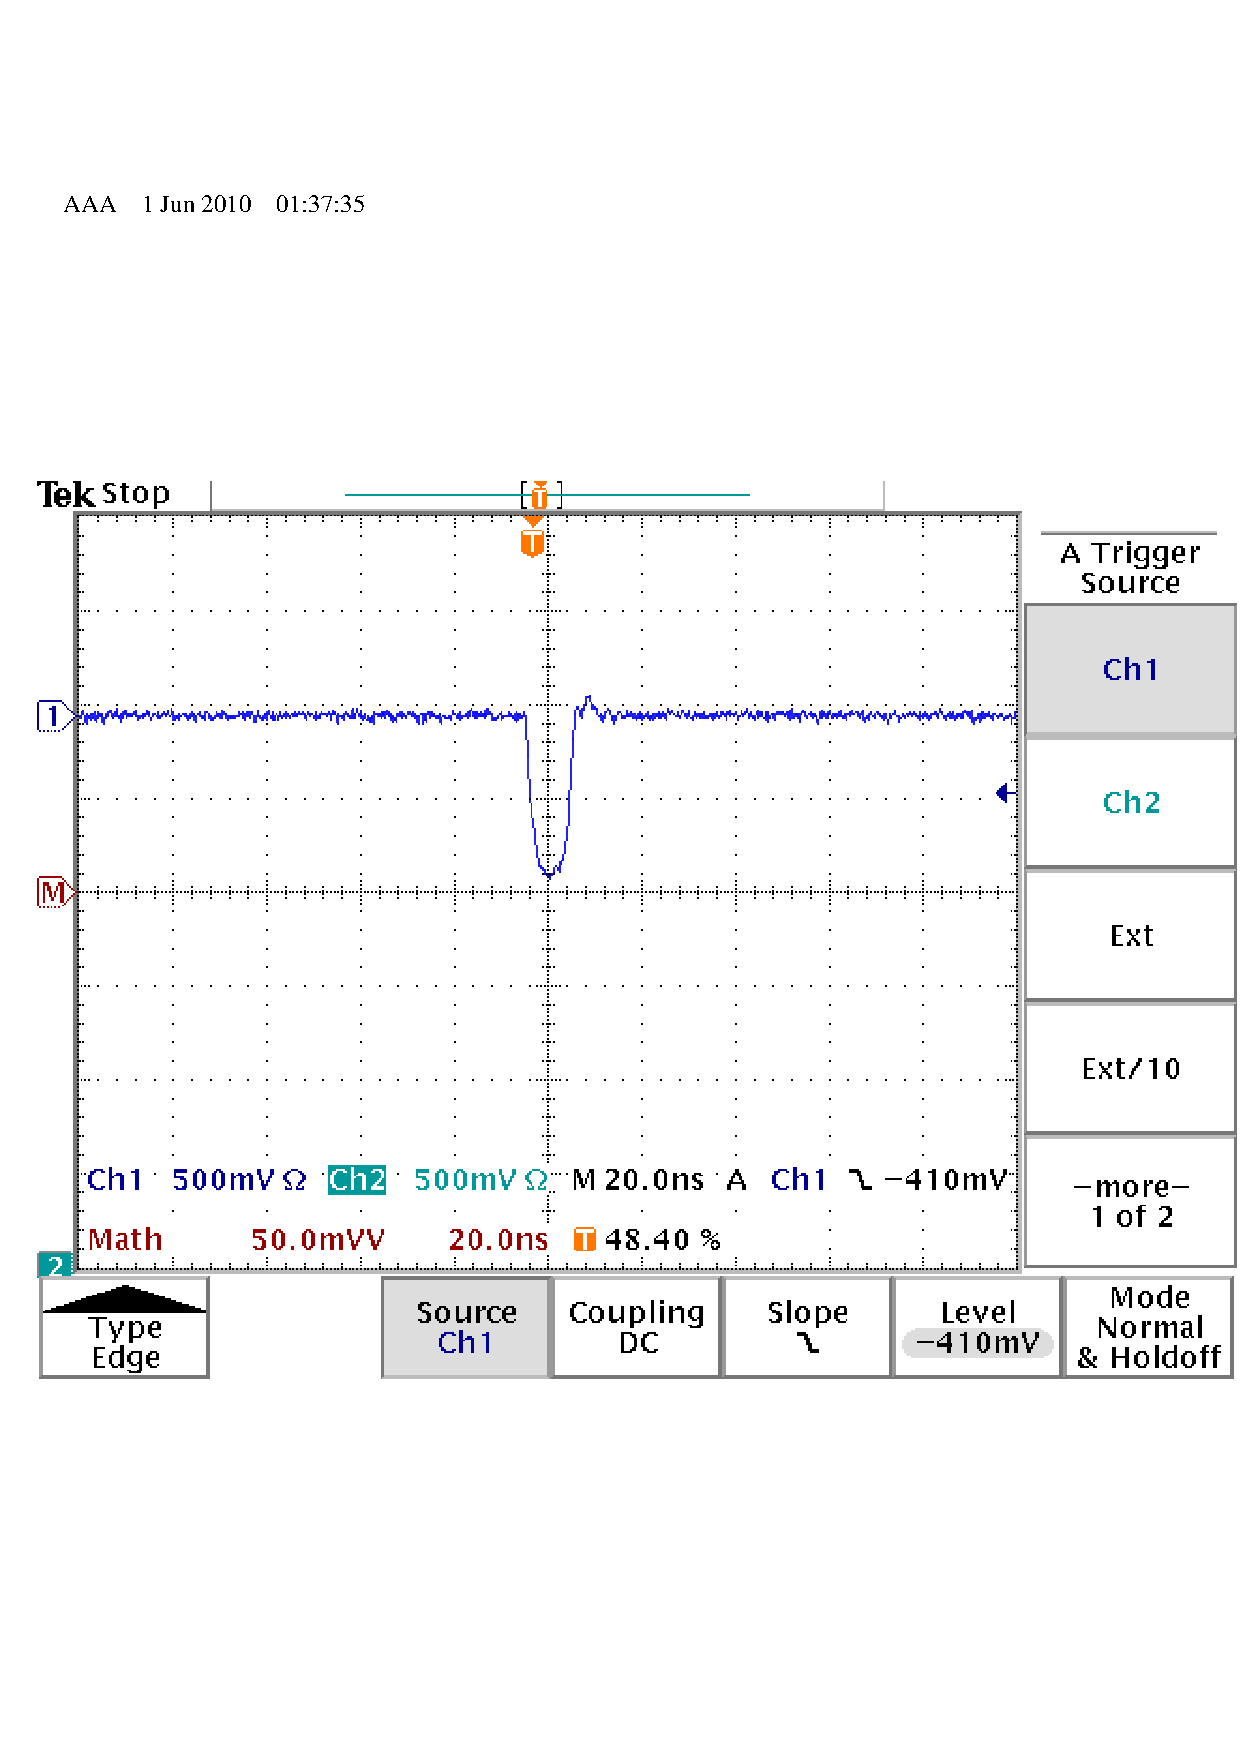
\includegraphics[width=0.45\textwidth,keepaspectratio,viewport=0 52 472 436,clip]{../tmp/TEK00015.pdf}
%   }
%   \subfloat[Photomultiplier 4]{
%     \label{fig:photomultiplier_4}
%     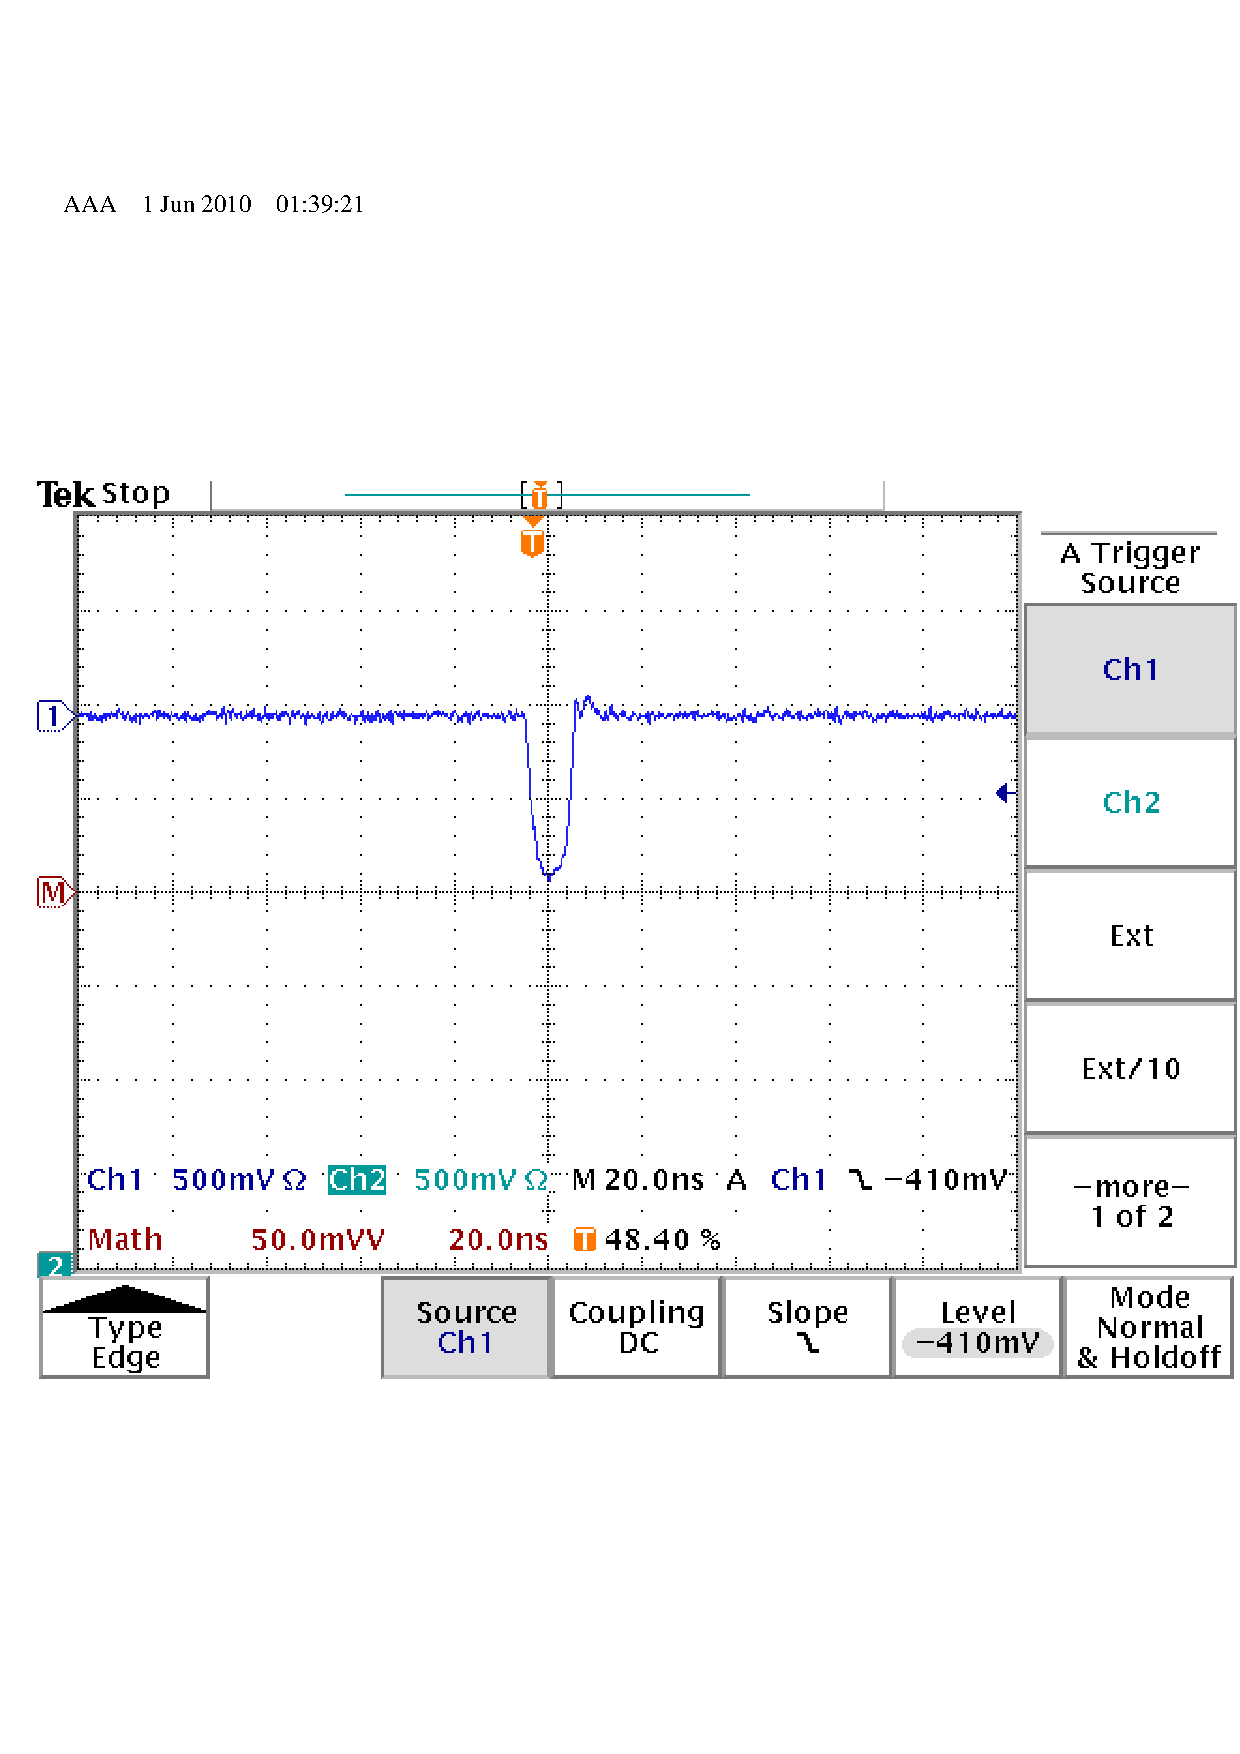
\includegraphics[width=0.45\textwidth,keepaspectratio,viewport=0 52 472 436,clip]{../tmp/TEK00016.pdf}
%   }
%   \newline
%   \subfloat[Photomultiplier 5]{
%     \label{fig:photomultiplier_5}
%     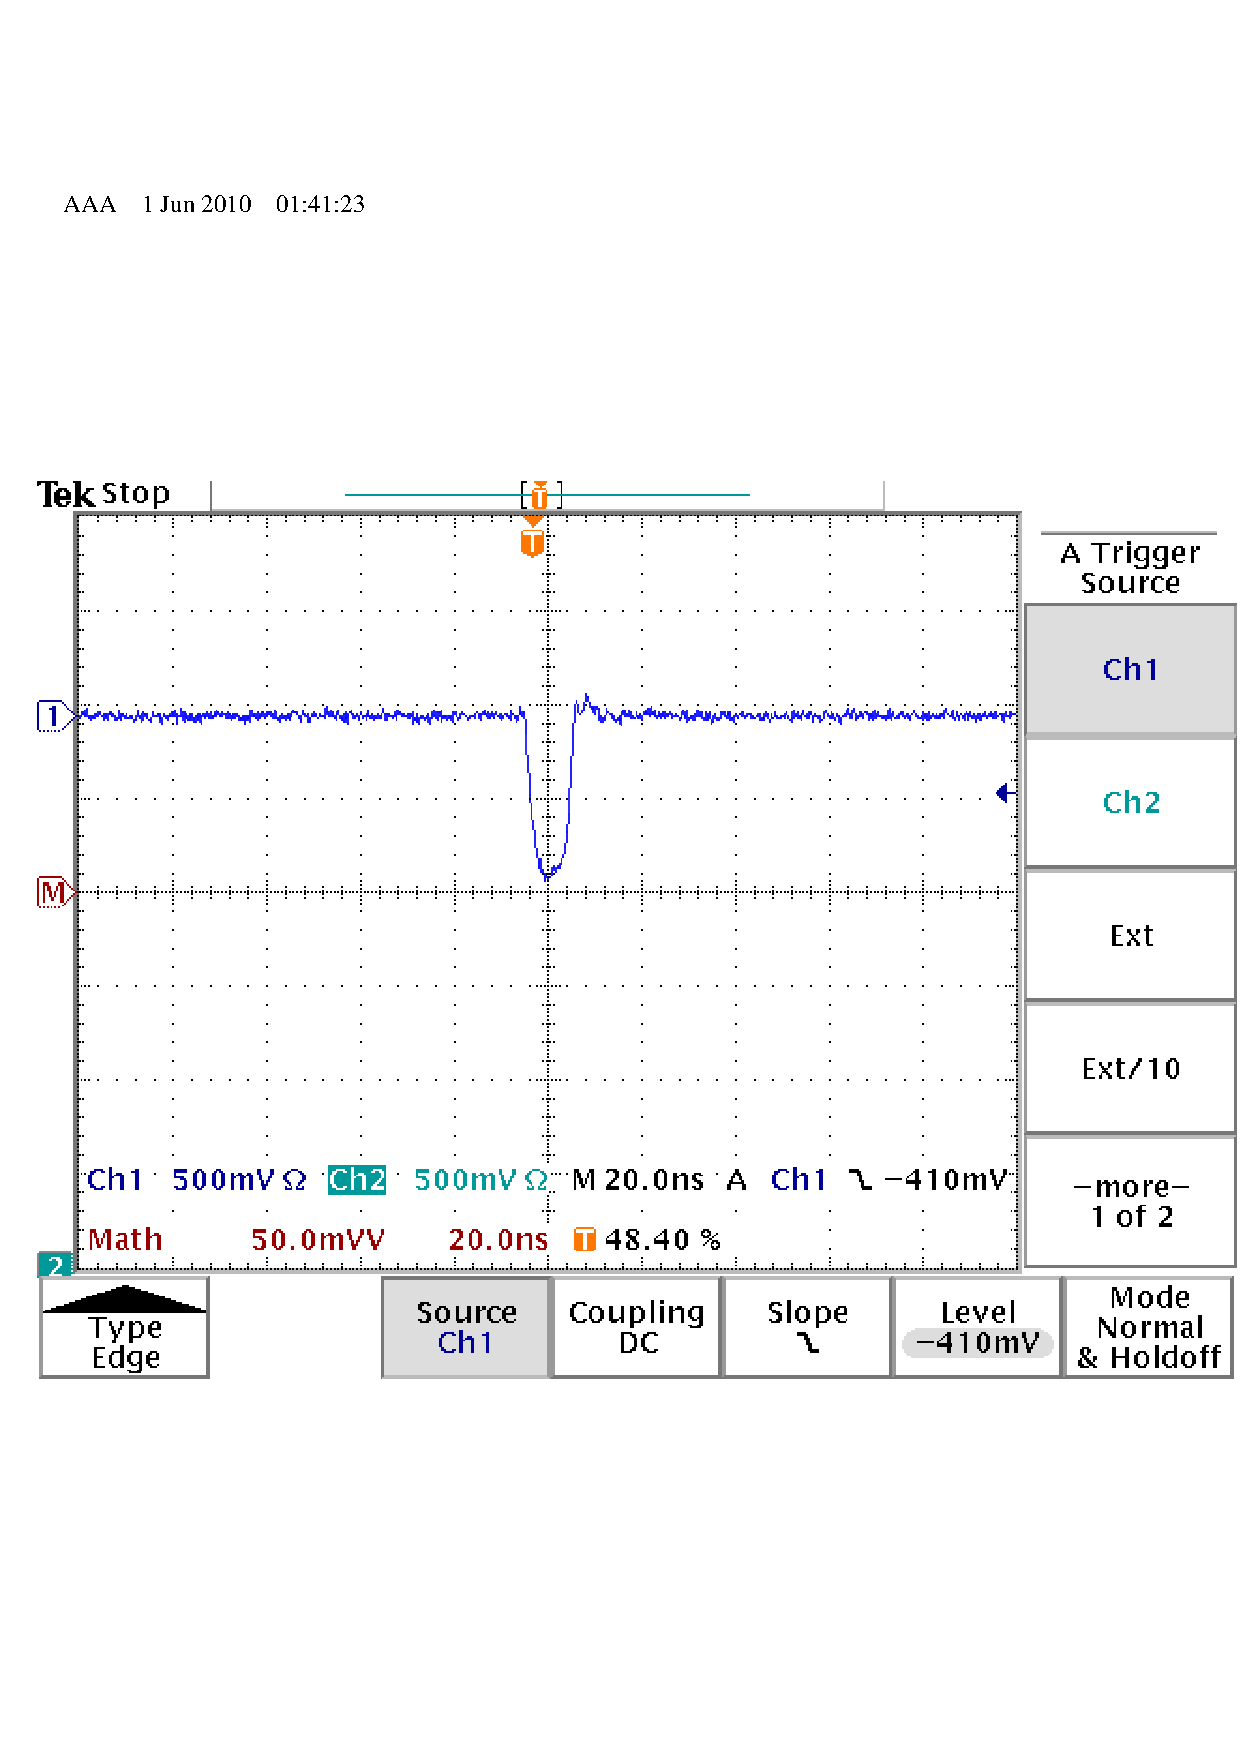
\includegraphics[width=0.45\textwidth,keepaspectratio,viewport=0 52 472 436,clip]{../tmp/TEK00017.pdf}
%   }
%   \caption{Signale in den einzelnen Photomultipliern}
%   \label{fig:PMs}
% \end{center}
% \end{figure}
